\chapter{Introduction}
\label{cpt:format}

% small blurb summary

\section{The APT}

The Advanced Particle-astrophysics telescope is designed to be a successor to the Fermi Gamma-ray Space Telescope, which has surpassed its expected mission time of 10 years. The main science objectives of the APT include studying high-energy transient phenomena such as supernovae and gamma-ray bursts (GRBs), continuing the search for dark matter, and conducting broader surveys of the sky in gamma rays. The APT would improve upon Fermi's sensitivity while maintaining a similar budget, allowing for a more extensive search for dark matter and an increased ability to detect transients.

\subsection{Hardware design}

The APT is designed to be used in the mid-keV to low TeV energy range, which is a significant improvement on Fermi's detecting range. The final telescope will consist of 20 repeated layers of detecting material, spaced 15 cm apart, in a cube 3 meters tall and 2.5 meters on each side. The middle section of each layer - the calorimeter - records the energy of each photon or particle that interacts with it, and the WLS fibers on the top and bottom of each layer record the corresponding position of each interaction. From this series of detected interactions, we are able to reconstruct the initial direction of the photon source using software.

\begin{figure}
    \centering
    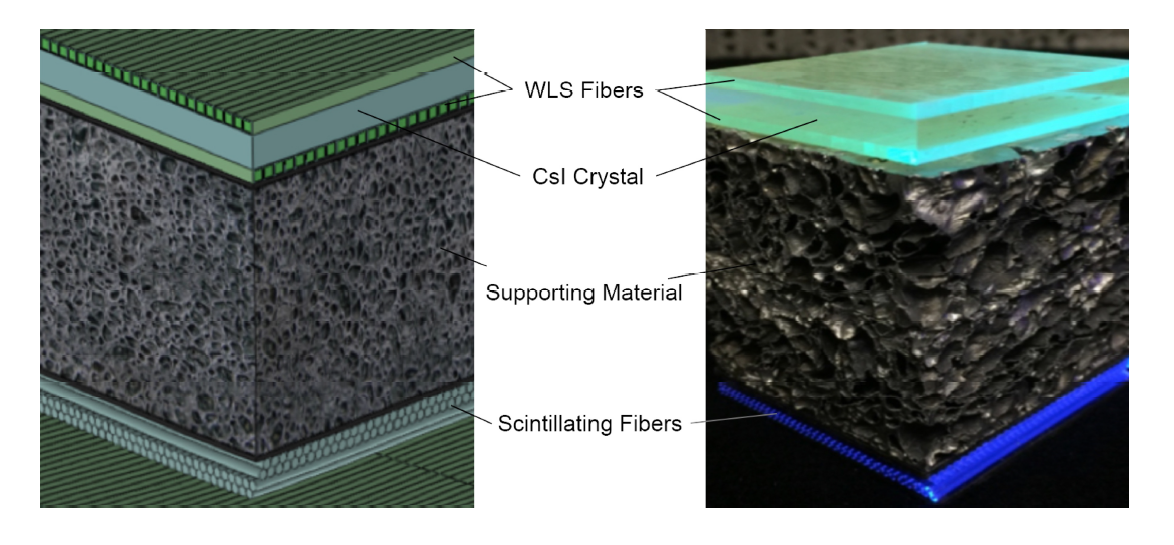
\includegraphics[width=0.7\textwidth]{APT_layers.png}
    \caption{One layer of the APT, shown as a computer model on the left and as a real-world prototype on the right, with aluminum used for the support structure. The Cesium Iodide (CsI) detects photon energy while the WLS fibers detect photon position. The scintillating fibers detect the position of any matter particles that enter the detector. Each subsequent layer would have the same structure as the one shown. \cite{APTmemo}}
    \label{fig:APT_layer}
\end{figure}

\subsection{Software design}
The APT achieves such a broad energy range by using two different software methods for reconstructing the trajectories of incoming photons, one for each of the two dominant gamma-ray interactions in this energy range. Below approximately 30 MeV, the dominant interaction is called Compton scattering, a process by which a photon transfers some portion of its momentum to an electron in a detector layer, changing its wavelength and trajectory. In the mid-MeV to GeV range, photons most commonly undergo a process called pair production upon interacting with the detector, in which a photon splits into a positron and an electron, which then interact further with the detector. As the goal of this project is to reconstruct Compton scatters, a thorough discussion of pair production is outside the scope of this paper, but a description of this phenomenon can be found in almost any particle physics textbook.

\section{Gamma-ray Bursts}
Though the APT can theoretically detect many types of transients, we focus primarily on gamma-ray bursts for this project. A gamma-ray burst (GRB) is an extremely bright burst of gamma-rays from a point source in the sky. These were first discovered in the 1960s by a US satellite that had been set up to detect radiation from nuclear blasts during the Cold War. The Compton Gamma-Ray Observatory (CGRO), launched in 1991, was used to determine that GRBs originate mainly from outside the Milky Way, and the Fermi Gamma-Ray Space Telescope, launched in 2008, has increased our understanding of the processes that cause these highly energetic blasts. A GRB can last anywhere from a few milliseconds to several hours, which is an incredibly short time window compared to most other astronomical observations. Many astrophysicists now believe that short-duration GRBs are caused by neutron-star mergers (collisions of extremely dense stellar remnants), while longer-duration GRBs originate from core-collapse supernovae (explosions of high mass stars), however much remains a mystery about how and why these events occur.

\section{This project}
\subsection{Motivation}
Though several theories exist as to their causes, the emission mechanisms of GRBs are not yet well-understood. The energies involved indicate a very efficient conversion of matter to energy, the process that drives this conversion is still an open question in the field of astrophysics. To better understand the processes that produce GRBs, it would be highly useful to observe them simultaneously with multiple different telescopes at multiple different wavelengths (gamma-ray, optical, infrared, etc.) To do this, we must be able to search for and detect a GRB in its initial stages and send out its location to other observatories. Achieving this goal could lead to future discovery in the field of astrophysics as GRBs become better understood.

One major science objective of the APT is to process gamma-ray events quickly enough to localize a source within a few seconds of the start of the burst and signal its location in that time. This means that we must significantly increase the detection capabilities of the APT in the low-energy range (keV - MeV) such that the incoming photons' directions can be reconstructed as quickly as they are received by the detector. As Compton scattering is the dominant interaction at these low energies, the primary focus of this research is to develop and test an algorithm to reconstruct Compton-scattered photons quickly and accurately enough that the telescope can pinpoint their source in close to real time. Many Compton telescopes rely on photon events with only two interactions to reconstruct their source positions. However, a significant fraction of events in this low energy range will scatter twice or more in the detector, which means that we can achieve significant performance improvement by incorporating the reconstruction of multi-scatter events into our algorithm.

\subsection{Scientific Constraints}

To eventually reach the main goal of this project, several factors be taken into account at this stage. The telescope must be able to reconstruct the trajectories of gamma rays at or near the speed at which they enter the detector, with low latency between the initial detection signal and the reconstructed solution. We expect to see between $10^5$ and $10^9$ photons per second during a typical gamma-ray burst\cite{UMD}. Our goal for reconstruction speed is $\backsim 10^5$ photons per second, with $>75\%$ accuracy and a latency of 1 second or less, as we expect this will give us an accurate enough localisation of the source position, but more complex simulations and source reconstructions will allow us to further constrain these target values. One of our other concerns is power consumption - the telescope will be part of a larger scientific instrument with a fixed amount of energy available to it daily. As such, we estimate that it cannot use more than 50 watts of power when running the reconstruction software.

\subsection{Process}
We base our initial Compton reconstruction algorithm on \emph{Boggs \& Jean (2000)}\cite{Boggs} and, with several performance improvements, we are able to meet our performance goals for this project. We start with a sequential algorithm, which enumerates each possible ordering of detector hits, and improve its performance by incorporating a tree search and pruning methods to improve the runtime. We build a simple gamma ray simulator for our development and initial tests of reconstruction speed and accuracy. Initial tests show that, with average parameters, the algorithm is able to reconstruct $\backsim 10^5$ photons per second with 80-90\% accuracy, which we believe will be enough to detect and localize a gamma-ray burst once the telescope is operational. By varying parameters in the algorithm, we also examine trends in the speed and accuracy, and discuss some possible trade-offs between the two, as well as possible improvements to the speed and accuracy for future work.

\section{Related Work}
One of the best papers available on Compton reconstruction procedures is \emph{Boggs \& Jean} (2000)\cite{Boggs} which details the mathematical formulae and steps required to reconstruct the initial direction of a Compton event in a layered detector. Though the paper focuses more on the physics of reconstructing Compton scatters than the algorithmic parameters, the equations listed served as a very helpful starting point for building and refining our code. We developed with the purpose of creating an algorithm to be as fast and lightweight as possible while still meeting our accuracy requirements. Many Compton telescopes must transfer data over a network connection or save observations in order to reconstruct them later, but our program is designed to process data in real time, before it leaves the telescope.

\iffalse
- Boggs \& Jean
        - focused more on the physics than the CS
        - Gives us a basic algorithm to improve upon
- Zoglauer's Megalib
- COMPTEL
    - It uses Compton scattering to detect GRBs, like our detector
    - But it only has two layers (lower probability of interaction) and as such it can only detect two-scatter events, a small fraction.
    - Has a good signal-to-noise ratio, which may be harder to emulate with the APT as it has a much larger detecting area
    - Might be more easy to determine polarization with more layers - Compton scattering is sensitive to photon polarization, so more Compton scatters would give us more chances to determine if the scattering angles have a preferential direction \cite{COMPTEL}.
    - It also has a Time Of Flight detector, which our telescope lacks
    - They also used Geant for testing
- COSI
    - It is also a multiple compton scattering detector
    - flies up on a balloon instead of being space-based
- MEGALib
    - basically the exact same thing as our algorithm but better
    - Realta package can reconstruct Compton events in real time
    - As far as I can tell, the only difference is you need an internet connection
\fi